\chapter{Interpretacja wyników}

W celu określenia jakości działania silnika kategoryzacyjnego przeprowadzono kilka testów. Testy polegały na przeprowadzeniu kategoryzacji obrazów pochodzących ze zbioru Caltech-101.\cite{CALTECH101}

Caltech-101 jest zbiorem obrazów przygotowanych na Kalifornijskim Uniwersytecie Technicznym (w skrócie \emph{Caltech}) przez Fei-Fei Li, Marca Andreetto oraz Marca Aurelio Ranzato. Zawiera obrazy nieobciążone ograniczeniami licencyjnymi podzielone na 101 kategorii.

Testy zostały przeprowadzone dla 2, 4 oraz 8 kategorii, dla zbiorów zawierających 1, 5, 10, 15, 20, 30 oraz 40 obrazów na kategorię. Poniżej znajdują się wykresy trafności dla poszczególnych przypadków.

\begin{figure}[h]
	\centering
	\includegraphics[scale=0.8]{graphics/04_interpretacja_wynikow/result-sift-2.pdf}
	\caption{ Wykres trafności dla uczenia 2 kategorii (SIFT) }
	\label{fig:result-sift-2}
\end{figure}

\begin{figure}[h]
	\centering
	\includegraphics[scale=0.8]{graphics/04_interpretacja_wynikow/result-sift-4.pdf}
	\caption{ Wykres trafności dla uczenia 4 kategorii (SIFT) }
	\label{fig:result-sift-4}
\end{figure}

\begin{figure}[h]
	\centering
	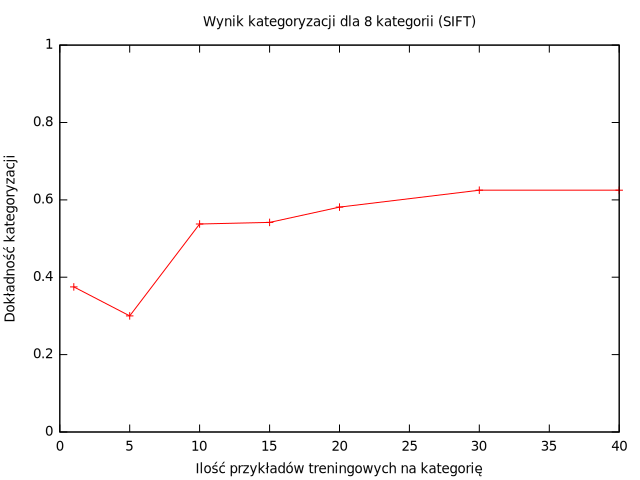
\includegraphics[scale=0.8]{graphics/04_interpretacja_wynikow/result-sift-8.pdf}
	\caption{ Wykres trafności dla uczenia 8 kategorii (SIFT) }
	\label{fig:result-sift-8}
\end{figure}

\begin{figure}[h]
	\centering
	\includegraphics[scale=0.8]{graphics/04_interpretacja_wynikow/result-surf-2.pdf}
	\caption{ Wykres trafności dla uczenia 2 kategorii (SURF) }
	\label{fig:result-sift-2}
\end{figure}

\begin{figure}[h]
	\centering
	\includegraphics[scale=0.8]{graphics/04_interpretacja_wynikow/result-surf-4.pdf}
	\caption{ Wykres trafności dla uczenia 4 kategorii (SURF) }
	\label{fig:result-sift-4}
\end{figure}

\begin{figure}[h]
	\centering
	\includegraphics[scale=0.8]{graphics/04_interpretacja_wynikow/result-surf-8.pdf}
	\caption{ Wykres trafności dla uczenia 8 kategorii (SURF) }
	\label{fig:result-sift-8}
\end{figure}